% VerA.web (public) Teχ-Experimente
%
% Copyright © 2015
%	Thorsten Glaser <t.glaser@tarent.de>
%
% Provided that these terms and disclaimer and all copyright notices
% are retained or reproduced in an accompanying document, permission
% is granted to deal in this work without restriction, including un‐
% limited rights to use, publicly perform, distribute, sell, modify,
% merge, give away, or sublicence.
%
% This work is provided “AS IS” and WITHOUT WARRANTY of any kind, to
% the utmost extent permitted by applicable law, neither express nor
% implied; without malicious intent or gross negligence. In no event
% may a licensor, author or contributor be held liable for indirect,
% direct, other damage, loss, or other issues arising in any way out
% of dealing in the work, even if advised of the possibility of such
% damage or existence of a defect, except proven that it results out
% of said person’s immediate fault when using the work as intended.

\documentclass{tarentanleitung}
\usepackage{tikz}
\usetikzlibrary{arrows,backgrounds,fit}
\begin{document}

% VerA.web (public) Installationsanleitung
%
% Copyright © 2015, 2016
%	Thorsten Glaser <t.glaser@tarent.de>
%
% Provided that these terms and disclaimer and all copyright notices
% are retained or reproduced in an accompanying document, permission
% is granted to deal in this work without restriction, including un‐
% limited rights to use, publicly perform, distribute, sell, modify,
% merge, give away, or sublicence.
%
% This work is provided “AS IS” and WITHOUT WARRANTY of any kind, to
% the utmost extent permitted by applicable law, neither express nor
% implied; without malicious intent or gross negligence. In no event
% may a licensor, author or contributor be held liable for indirect,
% direct, other damage, loss, or other issues arising in any way out
% of dealing in the work, even if advised of the possibility of such
% damage or existence of a defect, except proven that it results out
% of said person’s immediate fault when using the work as intended.

% VerA.web Fassung der Installationsanleitung
\newcommand{\vwiaversfassungnr}{4.2}
\newcommand{\vwiaversfassungmonat}{April}
\newcommand{\vwiaversfassungjahr}{2016}

% VerA.web Version
\newcommand{\vwiaverssw}{1.8.43}

% OSIAM Version (Auth-/Resource-Server, nicht Distribution)
\newcommand{\vwiaversosiam}{2.3}
% zugehörige Distribution
\newcommand{\vwiaversodist}{2.4}

% Upgrade von /etc/veraweb (1.4.3.5 oder 1.5.1.4+)
\newif\ifvwconfigsinetcalready
\vwconfigsinetcalreadyfalse

% Installationsanleitung oder nur Upgrade?
\newif\ifupgradeanleitung
\upgradeanleitungtrue

% Textweiche mit/ohne OA
\newif\ifoa
\oafalse

\tarentanleitung
 {Experimente}
 {\vwiaverspo}{\vwiaversfassungnr}{\vwiaversfassungmonat}{\vwiaversfassungjahr}{veraweblogo}

% LaTeX Table of Contents for tarent
%
% Copyright © 2015
%	Thorsten Glaser <t.glaser@tarent.de>
%
% Provided that these terms and disclaimer and all copyright notices
% are retained or reproduced in an accompanying document, permission
% is granted to deal in this work without restriction, including un‐
% limited rights to use, publicly perform, distribute, sell, modify,
% merge, give away, or sublicence.
%
% This work is provided “AS IS” and WITHOUT WARRANTY of any kind, to
% the utmost extent permitted by applicable law, neither express nor
% implied; without malicious intent or gross negligence. In no event
% may a licensor, author or contributor be held liable for indirect,
% direct, other damage, loss, or other issues arising in any way out
% of dealing in the work, even if advised of the possibility of such
% damage or existence of a defect, except proven that it results out
% of said person’s immediate fault when using the work as intended.
%-
% include with 「% LaTeX Table of Contents for tarent
%
% Copyright © 2015
%	Thorsten Glaser <t.glaser@tarent.de>
%
% Provided that these terms and disclaimer and all copyright notices
% are retained or reproduced in an accompanying document, permission
% is granted to deal in this work without restriction, including un‐
% limited rights to use, publicly perform, distribute, sell, modify,
% merge, give away, or sublicence.
%
% This work is provided “AS IS” and WITHOUT WARRANTY of any kind, to
% the utmost extent permitted by applicable law, neither express nor
% implied; without malicious intent or gross negligence. In no event
% may a licensor, author or contributor be held liable for indirect,
% direct, other damage, loss, or other issues arising in any way out
% of dealing in the work, even if advised of the possibility of such
% damage or existence of a defect, except proven that it results out
% of said person’s immediate fault when using the work as intended.
%-
% include with 「% LaTeX Table of Contents for tarent
%
% Copyright © 2015
%	Thorsten Glaser <t.glaser@tarent.de>
%
% Provided that these terms and disclaimer and all copyright notices
% are retained or reproduced in an accompanying document, permission
% is granted to deal in this work without restriction, including un‐
% limited rights to use, publicly perform, distribute, sell, modify,
% merge, give away, or sublicence.
%
% This work is provided “AS IS” and WITHOUT WARRANTY of any kind, to
% the utmost extent permitted by applicable law, neither express nor
% implied; without malicious intent or gross negligence. In no event
% may a licensor, author or contributor be held liable for indirect,
% direct, other damage, loss, or other issues arising in any way out
% of dealing in the work, even if advised of the possibility of such
% damage or existence of a defect, except proven that it results out
% of said person’s immediate fault when using the work as intended.
%-
% include with 「\input{toc.tex}」 after \tarentanleitung{…}…

\addtocontents{toc}{\protect\thispagestyle{fancy}}
\addtolength{\cftsubsecnumwidth}{0.5em}
\addtolength{\cftsubsubsecindent}{0.5em}
\renewcommand{\cftsecleader}{\cftdotfill{\cftdotsep}}
\hypersetup{linkcolor = black}
\tableofcontents
\hypersetup{linkcolor = blue}
\newpage
」 after \tarentanleitung{…}…

\addtocontents{toc}{\protect\thispagestyle{fancy}}
\addtolength{\cftsubsecnumwidth}{0.5em}
\addtolength{\cftsubsubsecindent}{0.5em}
\renewcommand{\cftsecleader}{\cftdotfill{\cftdotsep}}
\hypersetup{linkcolor = black}
\tableofcontents
\hypersetup{linkcolor = blue}
\newpage
」 after \tarentanleitung{…}…

\addtocontents{toc}{\protect\thispagestyle{fancy}}
\addtolength{\cftsubsecnumwidth}{0.5em}
\addtolength{\cftsubsubsecindent}{0.5em}
\renewcommand{\cftsecleader}{\cftdotfill{\cftdotsep}}
\hypersetup{linkcolor = black}
\tableofcontents
\hypersetup{linkcolor = blue}
\newpage


\section{Experimente}

\subsection{tikz/pgf}

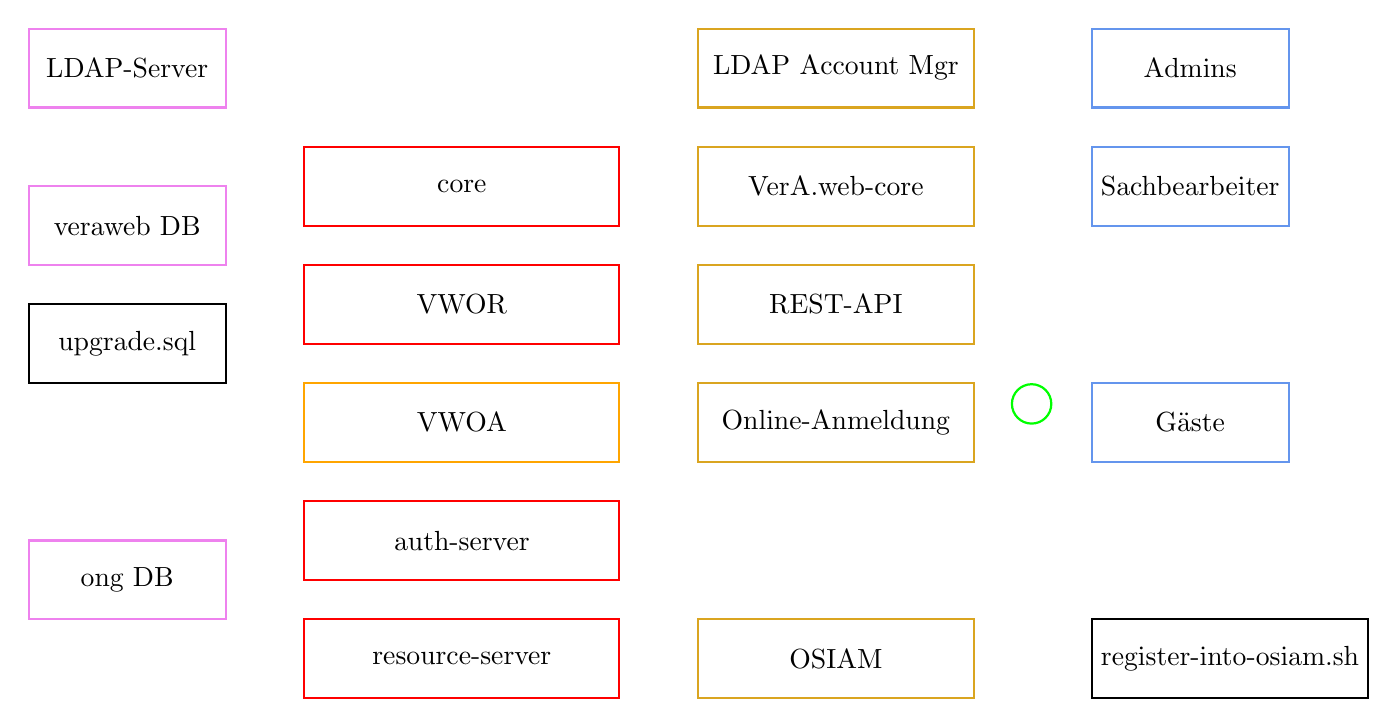
\begin{tikzpicture}[
  every node/.style={thick,text=black},
  every rectangle node/.style={above right,minimum height=10mm},
  apache/.style={rectangle,draw=Goldenrod,minimum width=35mm},
  microsvc/.style={rectangle,draw=Orange,minimum width=40mm},
  webapp/.style={rectangle,draw=red,minimum width=40mm},
  syssvc/.style={rectangle,draw=Violet,minimum width=25mm},
  script/.style={rectangle,draw=black,minimum width=25mm},
  people/.style={rectangle,draw=CornflowerBlue,minimum width=25mm},
  cloud/.style={circle,draw=green,minimum size=5mm},
 ]

  \node[apache]   (alam)   at ( 90mm,85mm) {LDAP Account Mgr};
  \node[apache]   (acore)  at ( 90mm,70mm) {VerA.web-core};
  \node[apache]   (avwor)  at ( 90mm,55mm) {REST-API};
  \node[apache]   (avwoa)  at ( 90mm,40mm) {Online-Anmeldung};
  \node[apache]   (aosiam) at ( 90mm,10mm) {OSIAM} [minimum height=25mm];
  \node[microsvc] (svwoa)  at ( 40mm,40mm) {VWOA};
  \node[webapp]   (score)  at ( 40mm,70mm) {core};
  \node[webapp]   (svwor)  at ( 40mm,55mm) {VWOR};
  \node[webapp]   (sauth)  at ( 40mm,25mm) {auth-server};
  \node[webapp]   (srsrc)  at ( 40mm,10mm) {resource-server};
  \node[syssvc]   (ldap)   at (  5mm,85mm) {LDAP-Server};
  \node[syssvc]   (dbvw)   at (  5mm,65mm) {veraweb DB};
  \node[syssvc]   (dbong)  at (  5mm,20mm) {ong DB};
  \node[script]   (usql)   at (  5mm,50mm) {upgrade.sql};
  \node[script]   (riosh)  at (140mm,10mm) {register-into-osiam.sh};
  \node[people]   (admins) at (140mm,85mm) {Admins};
  \node[people]   (sb)     at (140mm,70mm) {Sachbearbeiter};
  \node[people]   (guests) at (140mm,40mm) {Gäste};
  \node[cloud]    (inet)   at (132.5mm,47.5mm) {};


\end{tikzpicture}

\subsection{Seitenbreite}

Wie breit ist die Seite? % 497.92325pt ~= 175 mm (5 Nullen nach dem Komma)
% ein Teχ-Punkt (pt) ist exakt 2540/7227 mm = 0.3̅5̅1̅4̅5̅9̅8̅0̅ mm
% ein Teχ-Punkt (pt) ist exakt 800/803 PostScript-Punkt (pt, Teχ bp) = 0.9̅9̅6̅2̅6̅4̅0̅0̅ bp
% Teχ rechnet intern nur auf ca. 6 Stellen genau, fixed-point, daher vmtl. exakt

\the\textwidth

\subsection{bedingte Ausführung}

Kann ich Text ifdef'en?

\newif\ifosiam
\osiamtrue

\ifosiam
 OSIAM ja2 (ok)
\else
 OSIAM nein2
\fi

\ifosiam
 OSIAM ja1 (ok)
\fi

% \if!osiam ist immer false, \ifnotosiam schmeißt nen Fehler ☹
\ifosiam\else
 OSIAM nein1
\fi

\osiamfalse

\ifosiam
 OSIAM ja2
\else
 OSIAM nein2 (ok)
\fi

\ifosiam
 OSIAM ja1
\fi

% \if!osiam ist immer false, \ifnotosiam schmeißt nen Fehler ☹
\ifosiam\else
 OSIAM nein1 (ok)
\fi

\subsection{Abbildungen}

Gehen Abbildungen? Und wenn ja, wie macht man sie schön?

\begin{figure}[h!]
 \centering
\includegraphics[width=.8\textwidth]{veraweblogo}
% \\\the\textwidth % ändert sich nicht (getestet)
 \caption{Das Veraweb-Logo auf 80\% Breite}
 \label{fig:logovw}
\end{figure}

Hier könnte man noch etwas längeren Text einfügen, zum Beispiel
welchen, der erklärt, warum man hier eine Tilde \~{} statt eines
Leerzeichens verwendet, aber paßt schon so.

\newpage

Allerdings will ich den Umbruch und die Verweise testen, daher
brauche ich hier einen Seitenumbruch.

\begin{figure}[h!]
 \centering
\includegraphics[width=\textwidth]{tarentlogo}
% \\\the\textwidth
 \caption{Das tarent-Logo auf 100\% Breite}
 \label{fig:logotarent}
\end{figure}

In Abbildung~\ref{fig:logovw} sehen Sie das VerA.web-Logo;
Abbildung~\ref{fig:logotarent} verweist auf das neue tarent-Logo.

\subsection{Listing Copy \& Paste}

\begin{lstlisting}[language=sh,columns=fixed]
sudo mkdir -p /etc/veraweb/l10n
sudo install -c -o 0 -g 0 -m 644 l10n/* /etc/veraweb/l10n/
sudo install -c -o 0 -g 0 -m 644 config_ldap_access.xml /etc/veraweb/
sudo -u postgres createdb -E UTF-8 -O veraweb -T template0 veraweb

+---------------------------------------------------+
|                                                   |
| meh                                               |
| meow                                              |
| meh x                                             |
| ieh x                                             |
| iiiiiiiiiiiiiiiiiiiiiiiiiiiiiiiiiiiiiiiiiiiiiiiii |
| i     i     i     i     i       i       i       i |
| i i i i i i i i i i i i i i i i i i i i i i i i i |
| x x x x x x x x x x x x x x x x x x x x x x x x x |
| m m m m m m m m m m m m m m m m m m m m m m m m m |
| mmmmmmmmmmmmmmmmmmmmmmmmmmmmmmmmmmmmmmmmmmmmmmmmm |
| xxxxxxxxxxxxxxxxxxxxxxxxxxxxxxxxxxxxxxxxxxxxxxxxx |
| a!b"c#d$e%f&g'h(i)j*k+l-m/n^o_p`q~r\s[t{u|v?w^x<y |
| a b c d e f g h i j k l m n o p q r s t u v w x y |
+---------------------------------------------------+

\end{lstlisting}

\end{document}
